% Make nice A4 pages for print:
%\usepackage{pgfpages}
%\pgfpagesuselayout{resize to}[a4paper,border shrink=5mm,landscape]

\beamertemplatenavigationsymbolsempty

\setbeamertemplate{bibliography item}[text]

\usepackage[type={CC},modifier={by-sa},version={4.0}]{doclicense}

\usepackage[utf8]{inputenc}
\usepackage{hyperref}
\usepackage{breakurl}
\usepackage{graphicx}
\usepackage{pgfplots}
\usepackage{pgf}
\usepackage{tikz}
\usetikzlibrary{positioning}
\usetikzlibrary{arrows}
\usetikzlibrary{decorations.markings}
\usetikzlibrary{calc}
\usetikzlibrary{matrix}
\usetikzlibrary{shapes}
\usetikzlibrary{decorations.pathmorphing}
\usetikzlibrary{fit}
\usetikzlibrary{backgrounds}
\usetikzlibrary{plotmarks}
\usepackage{stmaryrd}
\usepackage{listings}
\usepackage{pdflscape}
\usepackage{perpage}
\usepackage{appendixnumberbeamer}

%\usepackage[thmmarks,amsmath,amsthm]{ntheorem} % already included in beamer
\usepackage{thm-restate}

\usepackage[sort&compress,numbers]{natbib}  % to be have \citet, \citeauthor, \citeyear

\MakePerPage{footnote}

\tikzstyle{o}=[r,ppBlue]
\tikzstyle{r}=[thick,rectangle,align=center]
\tikzstyle{t}=[r,ppTrans] %,font=\bfseries]
\tikzstyle{dd}=[densely dashed]
\tikzstyle{n}=[r,ppBlue]
\tikzstyle{p}=[r,ppRed]
\tikzstyle{ppRed}  =[draw=red,  fill=  red!20]
\tikzstyle{ppBlue} =[draw=blue, fill= blue!20]
\tikzstyle{ppGreen}=[draw=green,fill=green!20]
\tikzstyle{ppTrans}=[draw=none, fill=none]

\usetheme{Warsaw}

\useoutertheme[subsection=true]{smoothbars}
%\useoutertheme[subsection=false]{miniframes}

\definecolor{bblue}{HTML}{D7DF01}	% yellow-ish actually, for better black/white printing
\definecolor{rred}{HTML}{C0504D}
\definecolor{ggreen}{HTML}{9BBB59}
\definecolor{ppurple}{HTML}{9F4C7C}
\definecolor{lightgray}{rgb}{0.3,0.3,0.3}
\definecolor{lightergray}{rgb}{0.9,0.9,0.9}
\definecolor{UniBlue}{RGB}{83,121,170}

\DeclareTextFontCommand\textintro{\normalfont\bfseries\itshape} % nice!
\newcommand{\intro}[2][]
{%
	\textintro{#2}%
}
\newcommand{\empha}[2][]
{%
	\emph{#2}%
}

%\theoremstyle{plain}
\newcounter{reqcounter}
\newtheorem{requirement}[reqcounter]{Requirement}

%setbeamercolor{structure}{fg=violet}

\makeatletter
\def\th@task{%
    \normalfont % body font
    \setbeamercolor{block title example}{bg=orange,fg=white}
    \setbeamercolor{block body example}{bg=orange!20,fg=black}
    \def\inserttheoremblockenv{exampleblock}
  }
\makeatother

\theoremstyle{task}
\newtheorem{task}{Task}

\newenvironment{assignment}%
{%\setbeamercolor{background canvas}{bg=violet}%
%\setbeamercolor{structure}{fg=cyan!90!black}%
 \setbeamercolor{frametitle}{bg=orange,fg=white}
\begin{frame}}%
{\end{frame}}%

\AtBeginSection[]{
  \begin{frame}
  \vfill
  \centering
  \begin{beamercolorbox}[sep=8pt,center,shadow=true,rounded=true]{title}
    \usebeamerfont{title}\insertsectionhead\par%
  \end{beamercolorbox}
  \tableofcontents
  \vfill
  \end{frame}
}




\pgfplotsset{compat=1.14}
\author{Markus Raab}


\date{15.05.2019}

\begin{document}

\renewcommand{\enquote}[1]{\emph{``#1''}} % Cannot be done earlier

%%%%%%%%%%%%%%%%%%%%%%%%%%%%%%%
\begin{frame}
	\titlepage
	\doclicenseThis
\end{frame}


\begin{frame}
	Lecture is every week Wednesday 09:00 - 11:00.

	\begin{description}
		\item[06.03.2019:] {\color{gray}topic, teams}
		\item[13.03.2019:] {\color{gray}TISS registration, initial PR}
		\item[20.03.2019:] {\color{gray}other registrations, guest lecture}
		\item[27.03.2019:] {\color{gray}PR for first issue done, second started}
		\item[03.04.2019:] {\color{gray}first issue done, PR for second}
		\item[10.04.2019:] {\color{gray}mid-term submission of exercises}
		\item[08.05.2019:] {\color{gray}different location: Complang Libary}
		\item[15.05.2019:]
		\item[22.05.2019:] all 5 issues done
		\item[29.05.2019:]
		\item[05.06.2019:] final submission of exercises
		\item[12.06.2019:]
		\item[19.06.2019:] last corrections of exercises
		\item[26.06.2019:] exam
	\end{description}
\end{frame}

\begin{assignment}
	\frametitle{Tasks for today}
	(until 15.05.2019 23:59)

	\begin{task}
	Fourth PR done, PR for fifth issue created.
	\end{task}
\end{assignment}

\begin{assignment}
	\frametitle{Tasks for next week}
	(until 22.05.2019 23:59)

	\begin{task}
	All issues done.
	\end{task}

	\begin{task}
	Continue teamwork and homework.
	\end{task}
\end{assignment}

\begin{frame}
	\frametitle{Popular Topics}
	\vspace{-0.55cm}
	\setlength{\columnsep}{-1.3cm}
	\raggedright
	\begin{multicols}{2}
	\begin{description}
	\item[14] tools
	\item[9] {\color{red} testability}
	\item[9] {\color{orange} code-generation}
	\item[7] context-awareness
	\item[6] {\color{red} specification}
	\item[6] misconfiguration
	\item[6] {\color{gray} complexity reduction}
	\item[5] validation
	\item[5] {\color{red} points in time} % (early detection)
	\item[5] error messages
	\item[5] {\color{gray} auto-detection}
	\item[4] user interface
	\item[4] {\color{red} introspection}
	\item[4] design
	\item[4] cascading
	\item[4] {\color{red} architecture of access}
	\item[3] {\color{gray} configuration sources}
	\item[3] {\color{gray} config-less systems}
	\item[2] secure conf
	\item[2] {\color{gray} architectural decisions}
	\item[1] push vs.\ pull
	\item[1] infrastructure as code
	\item[1] full vs.\ partial
	\item[1] convention over conf %iguration
	\item[1] CI/CD
	\item[0] documentation
	\end{description}
	\end{multicols}
\end{frame}



\begin{frame}
	\frametitle{Goals for today}
	\textit{learning outcome:}
	\begin{itemize}
	\item evaluate a configuration system and decide about
	\begin{itemize}
	\item use of code generation (recapitulation)
	\item use of system-wide introspection
	\item testability
	\item time of validation
	\end{itemize}
	\end{itemize}
\end{frame}




%%%%%%%%%%%%%%%%%%%%%%%%%%%%%%%%%%%%%%%%%% 
\section{Introspection}

\subsection{}

\begin{frame}
	\frametitle{Introspection (Recapitulation)}
	\begin{alertblock}{Question}
	What can introspection offer?
	\end{alertblock}

	\pause
	\begin{itemize}
	\item unified get/set access to (meta*)-key/values
	\item access via applications, CLI, GUI, web-UI, ...
	\item access via any programming language (similar to file systems)
	\item GUI, web-UI can semantically interpret metadata
	\end{itemize}
\end{frame}

\begin{frame}[fragile]
	\frametitle{Internal Specification}

	For example, OWNER:
	\begin{code}[gobble=4,language=Java]
	import org.aeonbits.owner.Config;

	public interface ServerConfig extends Config {
		int port();
		String hostname();
		@DefaultValue("42")
		int maxThreads();
	}
	\end{code}
\end{frame}

\begin{frame}
	\begin{alertblock}{Question}
	Why do we need an external specification?
	\end{alertblock}

	\pause
	\vspace{1em}

	\textbf{Introspection}:
	\begin{itemize}
	\item needed as communication of producers and consumers of configuration
	\item the foundation for any advanced tooling like configuration management tools
	\item essential for \intro[no-futz computing]{no-futz computing}~\citet{holland2001nofutz}
	\end{itemize}
\end{frame}

\begin{frame}[fragile]
	\frametitle{External Specification}

	\begin{code}[gobble=4]
	[port]
	type:=long
	[hostname]
	default:=42
	[threads/max]
	type:=long
	\end{code}

	\vspace{1em}

	Advantages:
	\pause
	\begin{itemize}
	\item are read and writable by other applications (introspection)
	\item we can generate the internal specification (code generation)
	\item we fulfill needs for configuration management tools
	\end{itemize}
\end{frame}

\begin{frame}
	Other Artefacts (Recapitulation):

	\pause

	\begin{itemize}
	\item examples (e.g., defaults)
	\item documentation
	\item auto-completion/syntax highlighting/IDE support
	\item tooling (GUI, Web UI)
	\item validation code
	\item parsing code (e.g., command-line parsing)
	\item CM code
	\item configuration access APIs
	\end{itemize}
\end{frame}

\begin{frame}
	\frametitle{KeySet (Recapitulation)}

	The common data structure between plugins:
	\vspace{1cm}

	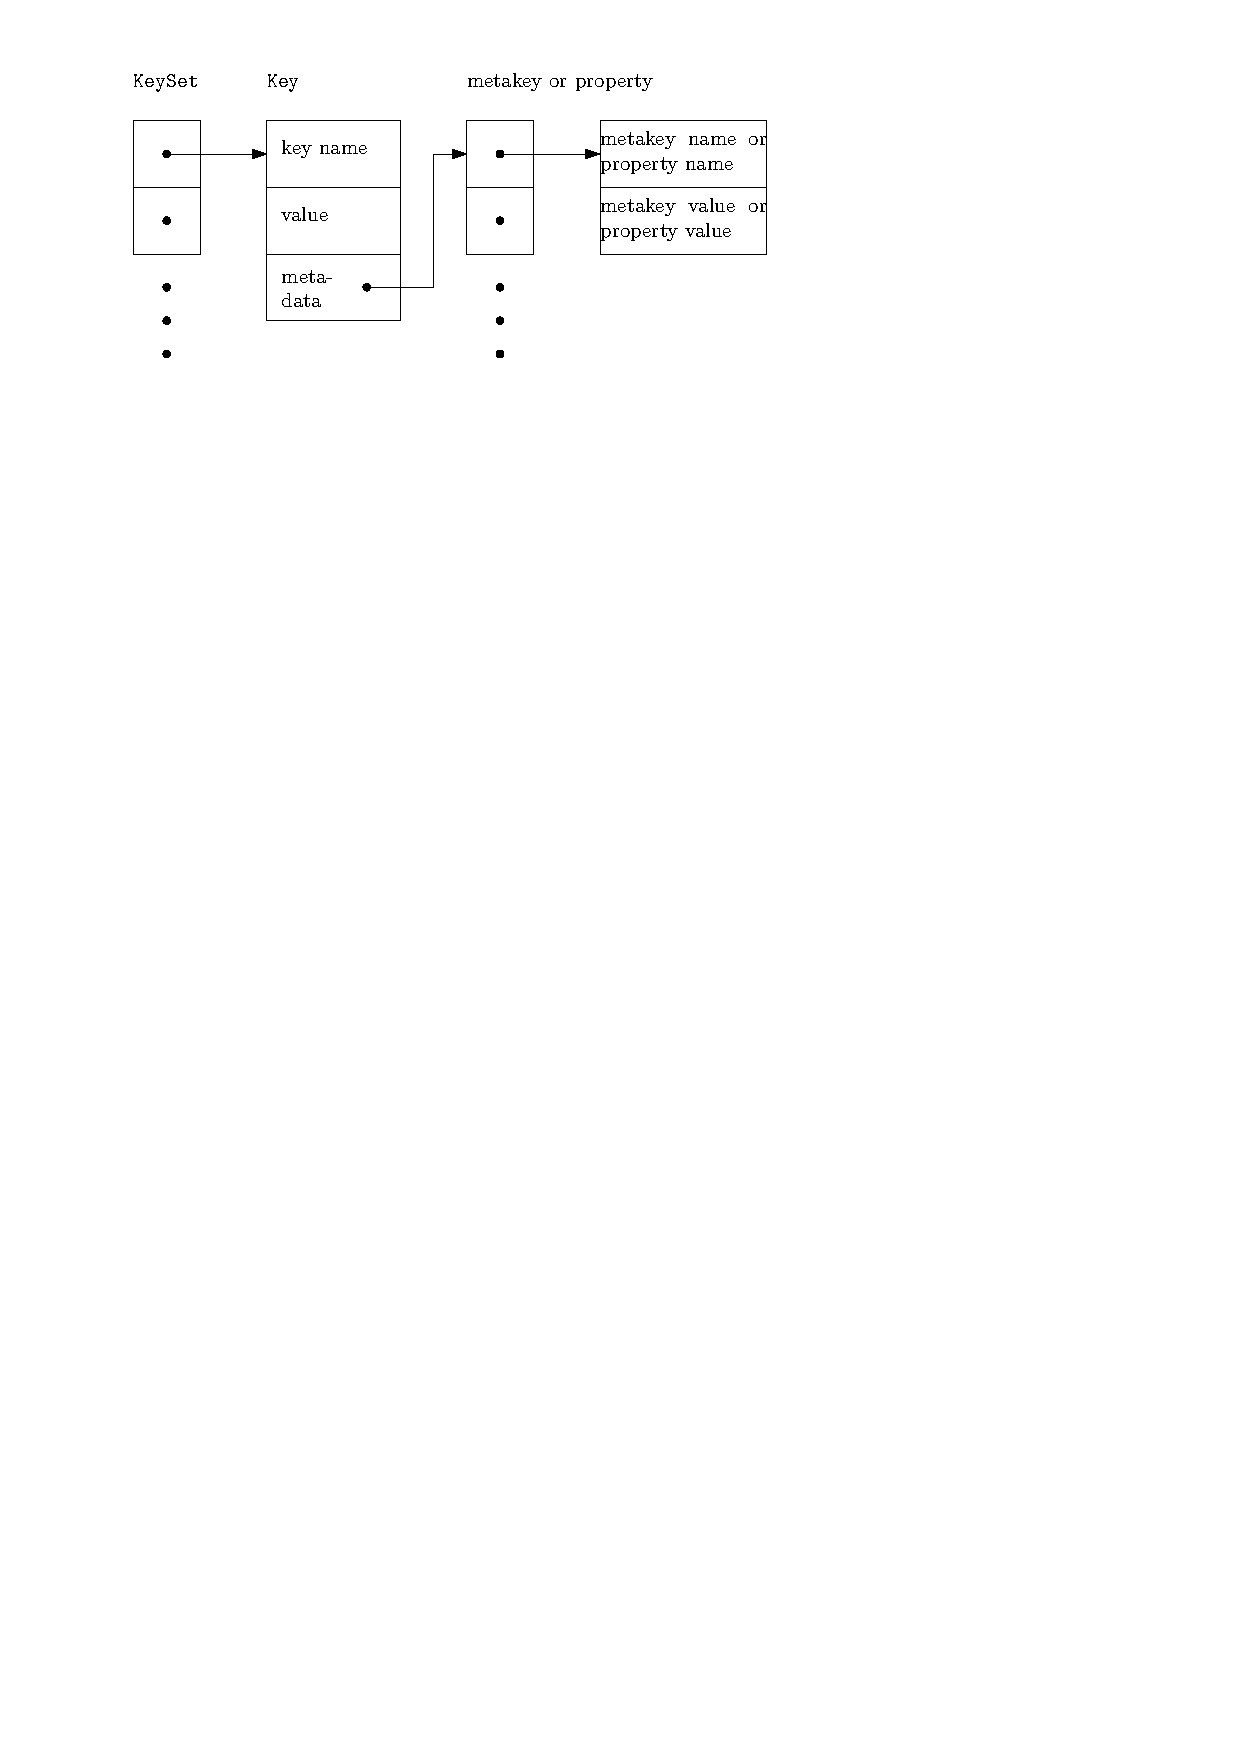
\includegraphics{keyset}
\end{frame}

\begin{frame}[fragile]
	\frametitle{KeySet Generation (Recapitulation)}
	\begin{alertblock}{Question}
	Idea: What if the configuration file format grammar describes source code?
	\end{alertblock}

	\pause

	key ^spec:/slapd/threads/listener^, with the configuration value ^4^ and the property $\property{default} \mapsto 1$:

	\begin{code}[gobble=4,language=Cpp]
	ksNew (keyNew ("spec:/slapd/threads/listener",
		       KEY_VALUE, "4",
		       KEY_META, "default", "1",
		       KEY_END),
	       KS_END);
	\end{code}

	\begin{alertblock}{Finding}
	We get source code representing the settings.
	\end{alertblock}
\end{frame}

\begin{frame}
	\frametitle{Possible Properties (Recapitulation)}

	\pause

	For example, SpecElektra has following properties:
	\begin{description}
	\item[type] represents the type to be used in the emitted source code.
	\item[opt] is used for short command-line options to be copied to the namespace \namespace{proc}.
	\item[opt/long] is used for long command-line options, which differ from short command-line options by supporting strings and not only characters.
	\item[restrict/write] yields compilation errors when developers assign a value to a contextual value within the program.
	\item[default] enables us to start the application even if the backend does not work.
	\end{description}
\end{frame}

\begin{frame}
	\frametitle{(Recapitulation)}
	\begin{alertblock}{Question}
	Introspection vs. Code Generation?
	\end{alertblock}

	\pause
	\vspace{0.5em}

	\setbeamersize{description width=1cm}
	\begin{description}
	\item[$-$] more techniques for performance improvements with code generation
	\item[$+$] specification can be updated live on the system without recompilation
	\item[$+$] tooling has generic access to all specifications
 	\item[$+$] new features the key database (e.g., better validation) are immediately available consistently
	\end{description}

	\vspace{0.5em}

	\begin{alertblock}{Implication}
	We generally prefer introspection, except for a very thin configuration access API.
	\end{alertblock}
\end{frame}



%%%%%%%%%%%%%%%%%%%%%%%%%%%%%%%%%%%%%%%%%% 
\section{Early Detection}

\subsection{}

\begin{frame}
	\frametitle{When are settings used?}
	\begin{description}[<+-| alert@+>]
	\item[Implementation-time] configuration accesses \index{implementation-time}
	are hard-coded settings in the sou\-rce code repository.
	For example, architectural decisions~\cite{zdun2007patterns} lead to impl\-ementation-time settings.

	\item[Compile-time] configuration accesses \index{compile-time}
	are configuration accesses resolved by the build system while compiling the code.

	\item[Deployment-time] configuration accesses \index{deployment-time}
	are configuration accesses while the software is installed.

	\item[Load-time] configuration accesses \index{load-time}
	are configuration accesses during the start of applications.

	\item[Run-time] configuration accesses \index{run-time}
	are configuration accesses during execution not limited to the startup procedure.
	\end{description}
\end{frame}

\begin{frame}
	\frametitle{Latent Misconfiguration}
	Phases when we can detect misconfigurations:
	\begin{itemize}[<+-| alert@+>]
	\item Compilation stage in configuration management tool
	\item Writing configuration settings on nodes
	\item Starting applications (load-time)
	\item When configuration setting is actually used (run-time)
	\end{itemize}

	\pause[\thebeamerpauses]

	\begin{alertblock}{Problem}
	More context vs. easier to detect and fix.
	\end{alertblock}
\end{frame}

\begin{frame}
	As shown by \citet{xu2016early}:
	\begin{itemize}[<+-| alert@+>]
	\item \p{12} -- \p{39} configuration settings are not used at all during initialization.
	\item Applications often have latent misconfigurations (\p{14} -- \p{93})
	\item Latent misconfigurations are particular severe (\p{75} of high-severity misconfigurations)
	\item Latent misconfiguration needs longer to diagnose
	\end{itemize}
\end{frame}

\begin{frame}
	\frametitle{Checkers as plugins}

	Using checkers as plugins exclude whole classes of errors such as:
	\begin{itemize}[<+-| alert@+>]
	\item Invalid file paths using the plugin \plugin{path}.
	\item Invalid IP addresses or host names using the plugins \plugin{network} or \plugin{ipaddr}.
	\end{itemize}

	\pause[\thebeamerpauses]
	Because the checks occur before the resources are actually used, the checks are subject to race conditions.\footnotemark
	\only<3->{\footnotetext[1]{For example, a path that was present during the check, can have been removed when the application tries to access it.}}

	\pause
	In some situations facilities of the operating system help\footnotemark, in others we have fundamental problems.\footnotemark
	\only<4>{\footnotetext[2]{For example, we open the file during the check and pass \texttt{/proc/<pid>/fd/<fd>} to the application. This file cannot be unlinked, but unfortunately the file descriptor requires resources.}}
	\only<4>{\footnotetext[3]{For example, if the host we want to reach has gone offline after validation.}}
\end{frame}

\begin{frame}[fragile]
	\frametitle{Example~\cite{xu2016early}}

	Squid uses ^diskd_program^ but not before requests are served.
	Latent misconfiguration caused 7h downtime and 48h diagnosis effort.

	\pause

	\begin{alertblock}{Finding}
	Configuration from all externals programs need to be checked, too.
	\end{alertblock}
\end{frame}


\begin{frame}
	\frametitle{Conclusion}

	\begin{itemize}[<+-| alert@+>]
	\item provide external specifications for other tooling and configuration management
	\item use code generation to keep internal specifications consistent with external specifications (e.g. for refactoring)
	\item implement checkers as plugins
	\item execute checkers as early as possible,
	also for external programs executed later
	\item keep important resources allocated after checking
	\end{itemize}

\end{frame}


\begin{frame}
	\frametitle{Preview}

	\begin{itemize}
	\item Documentation
	\item Notification
	\item Context-Awareness
	\end{itemize}
\end{frame}




%%%%%%%%%%%%%%%%%%%%%%%%%%%%%%%%%%%%%%%%%% 
\nocite{raab2017introducing}

\appendix

\begin{frame}[allowframebreaks]
	\bibliographystyle{plainnat}
	\bibliography{../shared/elektra.bib}
\end{frame}

\end{document}


